% Setup
\documentclass[a4 paper, 12pt]{memoir}

% Margins
\usepackage{geometry}
\geometry{margin=2cm}

% Title
\usepackage{fancyhdr}
\pagestyle{fancy}
%\setlength{\headheight}{20pt}
%\setlength{\footerheight}{20pt}
\fancyhf{}
\rhead{Teanlouise}
\lhead{COSC3000}
\cfoot{\thepage}

% Images
\usepackage{graphicx}
\usepackage{float}
\usepackage[export]{adjustbox}
\setlength{\intextsep}{5pt plus 2pt minus 2pt}

% Paragraph
\setlength{\parindent}{0em}
\setlength{\parskip}{0em}

% Text Formatting
\usepackage[utf8]{inputenc}
\usepackage[english]{babel}

% List spacing
\usepackage{enumitem}
\setlist{noitemsep, topsep=0pt}
\setlist[enumerate]{parsep=5pt} 

% Text Color
\usepackage{xcolor}

% Hyperlinks
\usepackage{hyperref}
\hypersetup{
    colorlinks=true,
    linkcolor=black,
    filecolor=black,      
    urlcolor=blue,
}

% Appendix
\usepackage{appendix}

% Include pdf
\usepackage{standalone}
\usepackage{pdfpages}

% Borders
\usepackage{mdframed}

%%%%%%%%%%%%%%%%%%%%%%%%%%%%%%%%%%%%%%%%%%
% DOCUMENT
\begin{document}
\begin{center}
    \Huge
\textbf{Visualisation Proposal}
\end{center}

\subsection*{What—what is the topic and goal of your project? }
The topic of this project is the Modern Olympics. The games have been a global competition since 1896 with both Summer and Winter sports. The goal is to analyse the patterns of a medal winner depending on their physical characteristics (weight, height, age, sex), home country (athleticism, GDP, population) and the games in which they compete (location).

% Body
\subsection*{Why—why is your project important and/or interesting? }
The Olympics are supposed to be a celebration of peace, inclusion and human persistence. It is an opportunity for people to be proud of their country, and be in awe of the feats of athletes. By exploring the above topics it may be possible to determine whether there is a fair representation at the Olympics, and whether the winners are too predictable. If this is the case than the Olympics are no longer serving their purpose.

\subsection*{How—how will you go achieve the goal of your project?}
The prediction of medal winners will be explored through a number of topics. Each of these will be presented as a comparison between the winter and summer games. Data will be considered from 1924 (when the Winter Olympics were introduced), except for BMI, GDP and population which will be taken from 1960 (when data is collected for majority of points for these variables). The variables ‘NOC’, ‘year’ and ‘season’ are used for all analysis. From current knowledge these are possible visualisations that can be explored:
    \begin{itemize}
        \item The distribution of the number of events and medals [Histogram (\#events, \#medal)]
        \item The change in age for medal and non-medal winners [Turkey box (year v. age)]
        \item The BMI of medal and non-medal winners [q-q plot (medal v. non-medal BMI)]
        \item The proportion of medal winners to number athletes [scatter (\#athletes v. \#medals)]
        \item The proportion of men and women competing [scatter (\#females v. \#males)]
        \item The difference in \% of medals when competing at host [scatter (\% hosting v. visiting)]
        \item The effect of population and GDP on number of medals [multi \- pop, GDP, \#medals]
    \end{itemize}


\subsection*{Data—what is your data source, how you will obtain it, and, if possible at this stage, provide a sample}

    \begin{enumerate}
        \item \underline{120 years of Olympic history (1896 - 2018)} - 
        Available for public download on Kaggle. Created by scraping \url{www.sport-reference.com}.
            \begin{itemize}
                \item noc\_regions.csv - A list of the countries and their code (at the time). 
                    \begin{figure}[H]
                        \centering
                        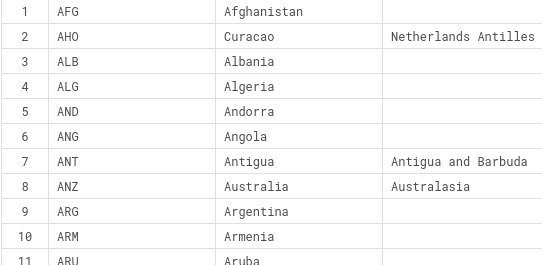
\includegraphics[width=0.6\textwidth, frame]
                            {./images/noc_data.png}                    
                    \end{figure}
                \item athlete\_events.csv \- Relevant information of all athletes. The variables of interest are ID, Sex, Age, Height, Weight, NOC, Year, Season, City, Medal.
                    \begin{figure} [H]
                        \centering
                        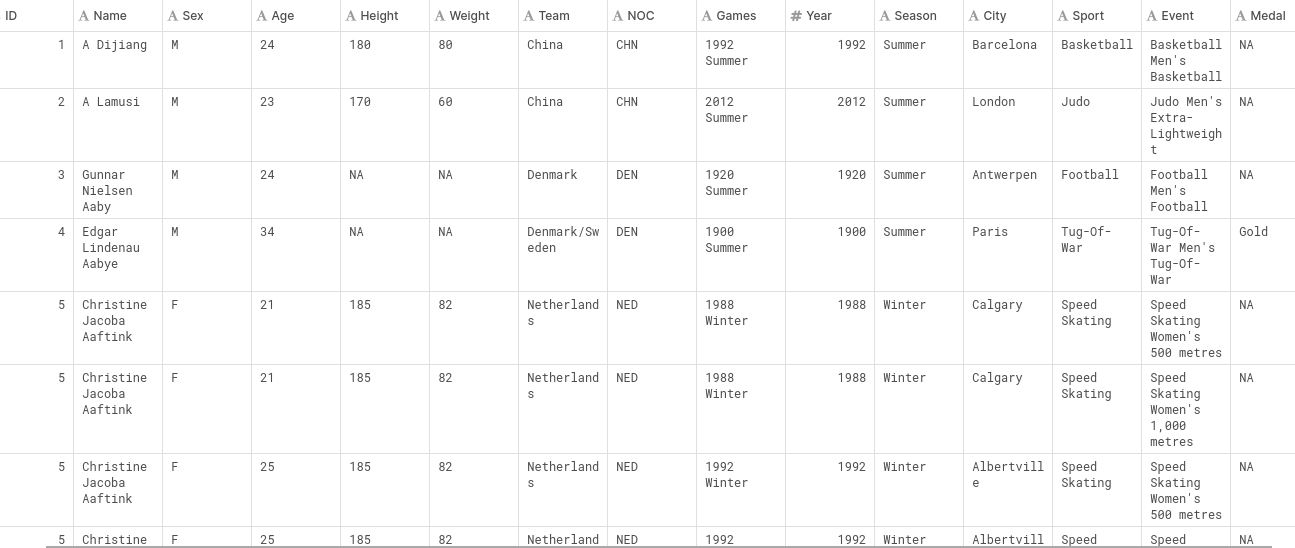
\includegraphics[width=\textwidth, frame]
                            {./images/history_data.png}                    
                    \end{figure}               
            \end{itemize}

        \item \underline{The World Bank (1960 - 2018)} - Available to the public from World Bank national accounts data, and OECD National Accounts data files.
            \begin{itemize}
                \item gdp.csv - The GDP for all countries, represented in current US\$.
                    \begin{figure} [H]
                        \centering
                        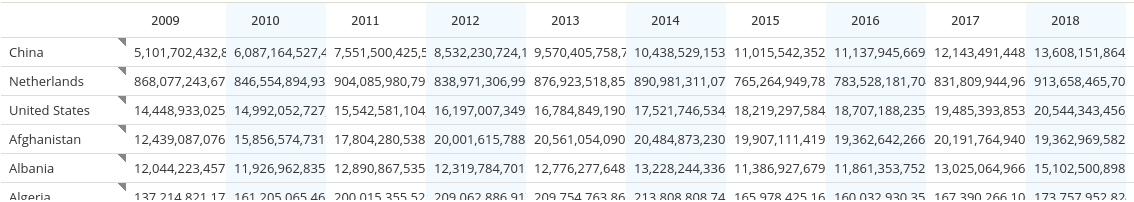
\includegraphics[width=\textwidth, frame]
                            {./images/gdp_data.png}                    
                    \end{figure}  
                \item population.csv - The total population of all countries
                    \begin{figure} [H]
                        \centering
                        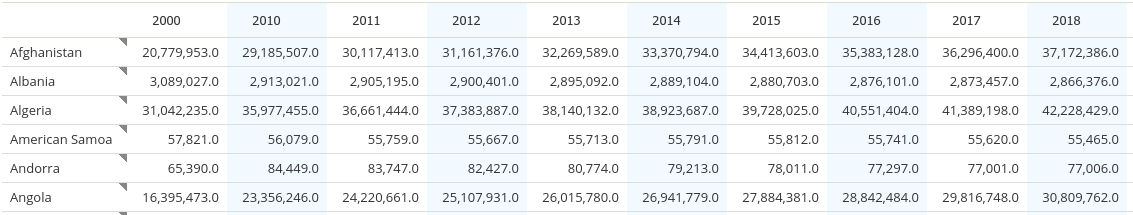
\includegraphics[width=\textwidth, frame]
                            {./images/pop_data.png}                    
                    \end{figure}  
            \end{itemize}
    
        \item \underline{List of Olympic Host Cities} - Manually create host\_city.csv of each games with city and country from \url{https://architectureofthegames.net/olympic-host-cities/}
            \begin{figure} [H]
                \centering
                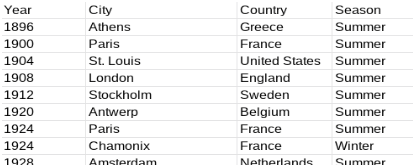
\includegraphics[width=0.6\textwidth, frame]
                    {./images/host_data.png}                    
            \end{figure}  
    \end{enumerate}
    
    \smallskip
    From these datasets a combined csv file will be created with all of the relevant variables.
    \begin{itemize}
        \item Remove ‘Name, Team, Games, Event’ \& Years 1896-1920 from athlete\_events.csv
        \item Add column COUNTRY by matching ‘NOC’ with the same from noc\_regions.csv
        \item Add column HOST COUNTRY by matching ‘country’ with same from host\_city.csv
        \item Add column GDP by matching ‘country’ in gdp.csv
        \item Add column POPULATION by matching ‘country’ in population.csv  
    \end{itemize}

    \begin{figure} [H]
        \centering
        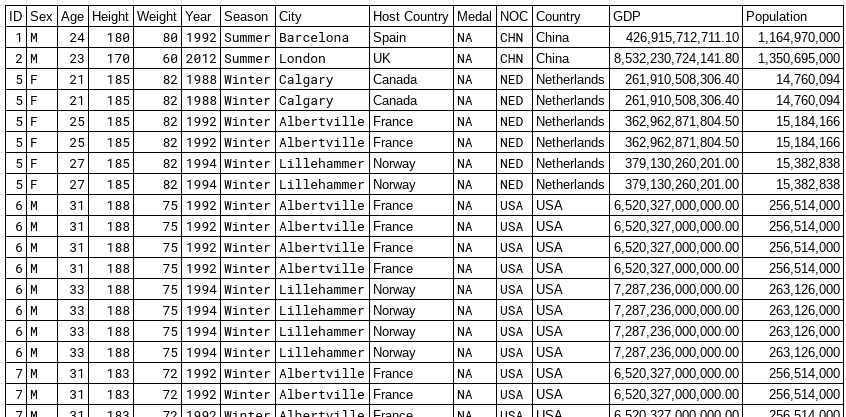
\includegraphics[width=\textwidth, frame]
            {./images/new_data.png}                    
    \end{figure} 


\subsection*{Notes—some important things to keep in mind during analysis}
    \begin{enumerate}
        \item athlete\_events.csv - Possible factors that may affect results of each Olympics
            \begin{itemize}
                \item 1924: Winter games commence
                1932: Low attendance due to Great Depression
                \item 1940 \& 1944: Cancelled due to WW2
                \item 1948: Art sports (architecture, literature, music, painting, sculpture) removed
                \item 1952: USSR/Russia starts competing, Republic of China (ROC) discontinued
                \item 1956: Boycotts by 8 nations, including China
                \item 1960: Height and Weight measured consistently from now
                \item 1976: Boycotts by 25 nations (mostly from Africa)
                \item 1980: Boycotts by 66 nations, including US
                \item 2000: Summer Olympics capped at 28 sports, 300 events, 10,000 athletes                
            \end{itemize}

        \item noc\_regions.csv - The following countries are recorded under multiple codes:
            
        \begin{itemize}
                \item Australia: AUS, ANZ (New Zealand, 1908\-1912)
                \item Russia: URS (1952\-1988), EUN (1992), RUS (1994\-2018)
                \item China: ROC (1924\-1948), CHN (1952\-2018), HKG (Hong Kong, 1952\-2018)
                \item Germany: GER (1896\-2018), EUA (1956\-1964), FRG \& GDR (1968\-1988)
                \item Czech Republic: CZE (1994\-2018), TCH (1920\-1992), BOH (1900\-1912)
                \item Serbia: SCG (2004\-2006), SRB (1912, 2008\-2018), YUG (1920\-2002)                    
            \end{itemize}  

    \end{enumerate}












\end{document}